\section{Week 3: Logic programming and ASP}

In \textbf{logic programming} you can express \textcolor{Maroon}{facts} and \textcolor{Maroon}{if-then rules}. Example: \textit{Prolog}. \textbf{Goal}: get computationally useful language to represent knowledge and reason with it. \\
\\
\textbf{Positive logic programs} consist of rules and facts (no negations and nots).
\begin{itemize}
    \setlength\itemsep{0em}
    \item \textbf{\textcolor{Maroon}{Rules}} are of the form (can all be true or false):
    \begin{lstlisting}
    a :- b, c, d, ..., z.
    \end{lstlisting}
    \hspace{0.75cm} which represents the implication \textcolor{NavyBlue}{$(b \wedge c \wedge d \wedge \ldots \wedge z) \rightarrow a$}
    \begin{itemize}
        \item \textbf{\textcolor{NavyBlue}{a}} is \textbf{\textcolor{NavyBlue}{head}} of the \textcolor{Maroon}{rule}.
        \item \textbf{\textcolor{NavyBlue}{$b, c, d, \ldots, z$}} is \textbf{\textcolor{NavyBlue}{body}} of the \textcolor{Maroon}{rule}.
    \end{itemize}
    \item \textbf{\textcolor{Maroon}{Facts}} are of the form:
    \begin{lstlisting}
    a.
    \end{lstlisting}
    \hspace{0.75cm} which represents the positive literal \textcolor{NavyBlue}{a}.
\end{itemize}

In \textbf{logic programming}, \textcolor{Maroon}{database semantics} is used:
\begin{itemize}
    \setlength\itemsep{0em}
    \item Objects mentioned are the only objects (\textbf{domain closure})
    \item Objects with different names are different objects (\textbf{unique-names assumption})
    \item (Atomic) statements that are not mentioned are false (\textbf{close-world assumption})
\end{itemize}

So we do not have to explicitly say what \textcolor{Maroon}{function symbols} mean. We can represent \textcolor{Maroon}{objects} simply by the terms that point to them. We can represent the meaning of a \textcolor{Maroon}{relation R} by the set of \textcolor{Maroon}{atoms (over R)} that are true-and then all atoms that are not in this set are false. \\
\\
For \textbf{positive logic programs}, there is a \textbf{\textcolor{Maroon}{unique minimal model}}:
\begin{itemize}
    \item \textcolor{Maroon}{Minimal} in terms of subset-inclusion
    \item \textcolor{Maroon}{Model} is an interpretation that makes all rules true
\end{itemize}

For example the \textcolor{Maroon}{minimal model} for the program below is: $\{a, b, c\}$:
\begin{lstlisting}
a :- b, c.
b :- c.
c.
d :- e.
\end{lstlisting}

We can find this \textbf{\textcolor{Maroon}{minimal model $M$}} with the following procedure:
\begin{enumerate}
    \setlength\itemsep{0em}
    \item Start by putting all facts of the program into $M$.
    \item Repeat until $M$ does not change anymore:\\
    If there is a rule $b \leftarrow c_1,\cdots,c_n$ where $c_1,\cdots,c_n \in M$ put $b$ in $M$ too.
\end{enumerate}

\textbf{Convention to}: write \textcolor{Maroon}{variables} starting with \textcolor{Maroon}{capital letters} and \textcolor{NavyBlue}{relation} and \textcolor{NavyBlue}{function symbols} starting with \textcolor{NavyBlue}{small letters}. \textcolor{Maroon}{Variables} are always \textcolor{Maroon}{universally quantified} ($\forall$).
\newpage

In \textbf{positive logic programs} it is \textbf{not allowed} to use \textcolor{Maroon}{negation} in the \textcolor{Maroon}{body} of rules (\textcolor{Maroon}{not}, which is $\neg$). However, some \textcolor{PineGreen}{extensions} allow this: \textbf{\textcolor{PineGreen}{Datalog}}.\\
\\
In \textbf{\textcolor{PineGreen}{Datalog}}, rules are of the following form:
\begin{lstlisting}
a :- $b_1$, ..., $b_n$, not $c_1$, ..., not $c_m$.
\end{lstlisting}

There are some \textcolor{Maroon}{restrictions} on programs:
\begin{itemize}
    \setlength\itemsep{0em}
    \item Function symbols (with arity $>$ 0) are not allowed
    \item Every variable that appears in the head of a rule, must also appear in a non-negated atom in the body.
    \item Every variable that appears in a negated atom in the body of a rule, must also appear in a non-negated atom in the body.
    \item Negation must be \textcolor{Maroon}{stratified}.
\end{itemize}

\textcolor{Maroon}{Negation} is \textcolor{Maroon}{stratified} in a program P if the following holds:
\begin{itemize}
    \setlength\itemsep{0em}
    \item Draw a directed graph, where the nodes are relation symbols appearing in P.
    \item For every rule $a \text{ :- } b_1, \ldots, b_n, \text{ not } c_1, \ldots, \text{ not } c_m$ in $P$:
    \begin{itemize}
        \item Draw an edge labelled with - (a \textcolor{Maroon}{negative edge}) from the relation symbol in \textcolor{Maroon}{a} to the relation symbol in \textcolor{Maroon}{$c_i$}, for each $1 \leq i \leq m$.
        \item Draw an edge labelled with + (a \textcolor{Maroon}{positive edge})  from the relation symbol in \textcolor{Maroon}{a} to the relation symbol in \textcolor{Maroon}{$b_i$}, for each $1 \leq i \leq n$.
    \end{itemize}
    \item If this graph has no cycles involving negative edges, then negation is \textcolor{Maroon}{stratified}.
\end{itemize}

\begin{figure}[ht!]
	\centering
	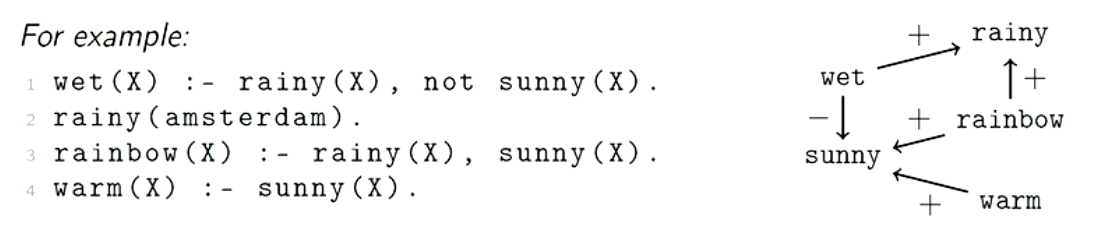
\includegraphics[scale=0.6]{figures/strat.png}
\end{figure}

\textbf{\textcolor{PineGreen}{Datalog}} programs have a \textcolor{Maroon}{unique minimal model} as well.
We can find it with the following procedure:
\begin{enumerate}
    \item Assign a \textcolor{Maroon}{positive integer} to each relation symbol such that: \\
    When there is a negative edge from \textcolor{Maroon}{a} to \textcolor{Maroon}{b}, then the number assigned to \textcolor{Maroon}{a} is strictly largert than that assigned to \textcolor{Maroon}{b} (since there are no cycles with negated edges).
    \item Start by putting all facts of the program into M.
    \item Proceed in stages, one stage for each assigned integer $i$, going from low to high. In each stage $i$:
    \begin{itemize}
        \item Repeat until $M$ does not change anymore: \\
        If there is a rule \textcolor{NavyBlue}{$b \leftarrow c_1, \ldots, c_n \text{ not } d_1, \ldots, \text{ not } d_m$} in $P$ where $c_1, \ldots, c_n \in M$ and $d_1, \ldots, d_m \not \in$, \textcolor{Maroon}{and b is assigned the number $i$}, then put $b$ in $M$ too.
    \end{itemize}
\end{enumerate}

\subsection{Answer Set Programming (ASP)}
What if we want to use negation, but it is not stratified in our knowledge base (\textcolor{Maroon}{unstratified negation})?\\
\\
For example:
\begin{lstlisting}
low :- not high.
high :- not low.
\end{lstlisting}

Then there is \textcolor{Maroon}{not always} a \textcolor{Maroon}{unique minimal model}. In this example, the following are (subset-) minimal models: $\{$low$\}$ and $\{$high$\}$.

\textbf{\textcolor{Maroon}{Answer Set Programming (ASP)}} assigns the so-called \textcolor{Maroon}{answer set semantics} to logic programs with negations. \\
\\
In the basic language of ASP, programs may contain facts and rules of the form:
\begin{lstlisting}
a :- $b_1$, ..., $b_n$, not $c_1$, ..., not $c_m$.
\end{lstlisting}
\begin{itemize}
    \item \textcolor{Maroon}{Negation} does \textcolor{Maroon}{not} have to be \textcolor{Maroon}{stratified}.
    \item It may contain variables, that must appear \textcolor{Maroon}{safely}:
    \begin{itemize}
        \item Every variable that appears in the head of a rule, must also appear in a non-negated atom in the body
        \item Every variable that appears in a negated atom in the body of a rule, must also appear in a non-negated atom in the body.
    \end{itemize}
\end{itemize}

\textbf{Semantics of ASP (intuitions)}:
\begin{enumerate}
    \setlength\itemsep{-0.5em}
    \item Consider an \textcolor{NavyBlue}{interpration M} as \textcolor{Maroon}{an assumption} for which atoms are true and which are false.
    \item Construct a (positive) \textcolor{NavyBlue}{variant $P^M$} of the program $P$ that takes into account this assumption.
    \item Check whether $M$ is the \textcolor{Maroon}{(unique) minimal model of $P^M$}.
\end{enumerate}

\begin{minipage}{0.5\textwidth}
Take a \textcolor{PineGreen}{normal logic program $P$} and an \textcolor{PineGreen}{interpretation $M$}.
\begin{itemize}
    \item The \textcolor{Maroon}{reduct $P^M$} of $P$ w.r.t. $M$ is obtained from $P$ by:
    \begin{enumerate}
        \item removing rules with \textcolor{MidnightBlue}{not a} in the body, for $a \in M$
        \item removing literals \textcolor{MidnightBlue}{not b} from all rules, for $b \not \in M$
    \end{enumerate}
    \item An \textcolor{Maroon}{answer set of $P$} is a set $M$ that is the minimal model of $P^M$.
\end{itemize}
\end{minipage}
\begin{minipage}{0.5\textwidth}
\centering
For example, take \textcolor{MidnightBlue}{$P$} to be: \\
\vspace{0.25cm}
\text{low} :- \text{not high}. \\
\text{high} :- \text{not low}. \\
\vspace{0.25cm}
% \end{lstlisting}
and \textcolor{MidnightBlue}{$M = \{ \text{high} \}$}. Then $P^M$ is: \\
\vspace{0.25cm}
high.\\
\vspace{0.25cm}
and $M$ is the minimal model of $P^M$.
\end{minipage}

\begin{minipage}{0.5\textwidth}
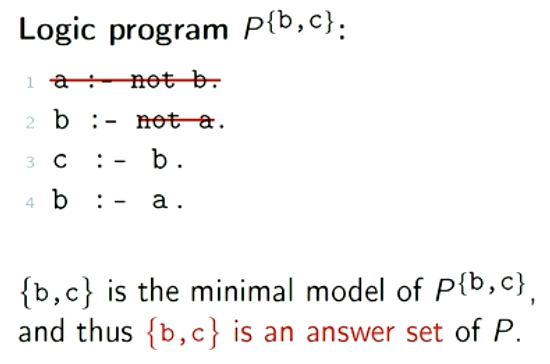
\includegraphics[scale=0.75]{figures/asp1.png}
\end{minipage}
\begin{minipage}{0.5\textwidth}
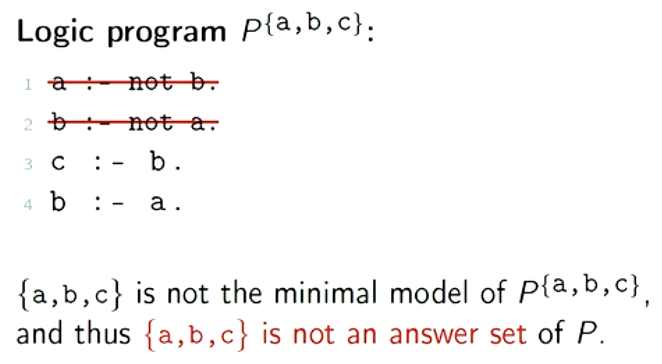
\includegraphics[scale=0.75]{figures/asp2.png}
\end{minipage}

\vspace{0.5cm}

In the figures above:
For any 2 answer sets of a program, they cannot be subsets of each other. The left figure shows that $\{b,c\}$ is an \textcolor{Maroon}{answer set}, which means that $\{a,b,c\}$ cannot be an answer set anymore. \\
\\
Some clarifications:
\begin{itemize}
    \item The first rule in the \textbf{left figure} gets thrown out completely. This is because when building the \textcolor{Maroon}{reduct}, we only look at the literals with \textcolor{Maroon}{not}. So for every \textcolor{Maroon}{not} \textit{something}, where \textit{something} is in the set $P^M$, that rule gets thrown out completely.
    \item In the second rule of the \textbf{left figure} only the right part of the rule gets striked, since we again look at \textcolor{Maroon}{not} \textit{something}, but \textit{something} is not in the set $P^M$. Thus we strike \textbf{not \textit{something}} in that rule.
    \item Thereafter we do the iterative procedure and see that $\{b,c\}$ is the answer set of $P$.
    \item In the \textbf{right figure} we go through the same procedure, except that $\{a,b,c\}$ is not an answer set, since it not the minimal model of $P^{\{a,b,c\}}$
\end{itemize}

\subsection{Building blocks of ASP (- check other PDF)}
\begin{minipage}{0.5\textwidth}
\textbf{Logic program with constraint}:
\begin{lstlisting}
num(1).
num(2).

left(X) :- not right(X), num(X).
right(X) :- not left(X), num(X).

:- left(1), left(2). $\;\;\;\;\;  \text{\textcolor{PineGreen}{\# left(1) and left(2) cannot be true both}}.$
\end{lstlisting}
\end{minipage}
\begin{minipage}{0.5\textwidth}
\textbf{Answer sets (because of constraint)}:
\begin{lstlisting}
num(1) num(2) right(1) left(2)
num(1) num(2) right(1) right(2)
num(1) num(2) left(1) right(2)



.
\end{lstlisting}
\end{minipage}

\vspace{0.25cm}
\textbf{Helpful feature: \# show}: \\
If you want to see a specific part (subset) of the answer set (not changing the problem or answer). 

\newpage
\textbf{Helpful feature: abbreviations}: \\
num(1..3) is equivalent to: num(1). num(2). num(3).  \\
\\
num(a;c) is equivalent to: num(a). num(c). \textbf{So not up to!} \\

\vspace{0.25cm}
\textbf{Helpful feature: \#const}: \\
A constant. So for example \#const k=2 and thereafter num(1, k) will give num(1) up to num(k). \\
\\
\textbf{Choice rules}: \\
Logic program:
\begin{lstlisting}
{ a; b }.
\end{lstlisting}

\begin{minipage}{0.5\textwidth}
Possible translation:
\begin{lstlisting}
a :- not na.
na :- not a.
b :- not nb.
nb :- not b.
\end{lstlisting}
\end{minipage}
\begin{minipage}{0.5\textwidth}
Answer sets:
\begin{lstlisting}
na nb
a nb
na b
a b
\end{lstlisting}
\end{minipage}

\textbf{Choice rule \textcolor{Maroon}{with lower bound}} (choose at least 2 of them): 
\begin{lstlisting}
2 { a; b; c }
\end{lstlisting}
So the anwser set becomes: a b, a c, b c and a b c.\\

\textbf{Choice rule \textcolor{Maroon}{with upper bound}} (choose at most 1 of them): 
\begin{lstlisting}
{ a; b; c } 1
\end{lstlisting}
So the anwser set becomes: \{empty answer set\}, a, and b. \\

\textbf{Choice rule \textcolor{Maroon}{with lower and upper bound}} (choose exactly 2 of them): 
\begin{lstlisting}
2 { a; b; c } 2
\end{lstlisting}
So the anwser set becomes: a b, a c, and b c. \\
\\


{\Large \textbf{\textcolor{Maroon}{Conditional literals (1)}}}: \\
\begin{minipage}{0.6\textwidth}
\textbf{Logic program}:
\begin{lstlisting}
p(1..3).
q(1..2).
s :- p(X) : q(X)
\end{lstlisting}
\end{minipage}
\begin{minipage}{0.3\textwidth}
\textbf{Answer sets}:
\begin{lstlisting}
p(1) p(2) p(3) q(1) q(2) s

.
\end{lstlisting}
\end{minipage}

\newpage

{\Large \textbf{\textcolor{Maroon}{Conditional literals (2)}}}: \\
\begin{minipage}{0.4\textwidth}
\textbf{Logic program}:
\begin{lstlisting}
p(1..3).
q(1..2).
r(1..3).
s :- p(X) : q(X), r(X)
\end{lstlisting}
\end{minipage}
\begin{minipage}{0.6\textwidth}
\textbf{Answer sets}:
\begin{lstlisting}
p(1) p(2) p(3) q(1) q(2) r(1) r(2) r(3) s


.
\end{lstlisting}
\end{minipage}

\vspace{0.35cm}

{\Large \textbf{\textcolor{Maroon}{Conditional literals (3)}}}: \\
\begin{minipage}{0.4\textwidth}
\textbf{Logic program}:
\begin{lstlisting}
p(1..3).
q(1..2).
r(1..3).
t.
s :- p(X) : q(X), r(X) ; t
\end{lstlisting}
\end{minipage}
\begin{minipage}{0.6\textwidth}
\textbf{Answer sets}:
\begin{lstlisting}
p(1) p(2) p(3) q(1) q(2) r(1) r(2) r(3) s t



.
\end{lstlisting}
\end{minipage}

\vspace{0.35cm}

{\Large \textbf{\textcolor{Maroon}{One-to-one mappings}}}: 
\begin{figure}[ht!]
    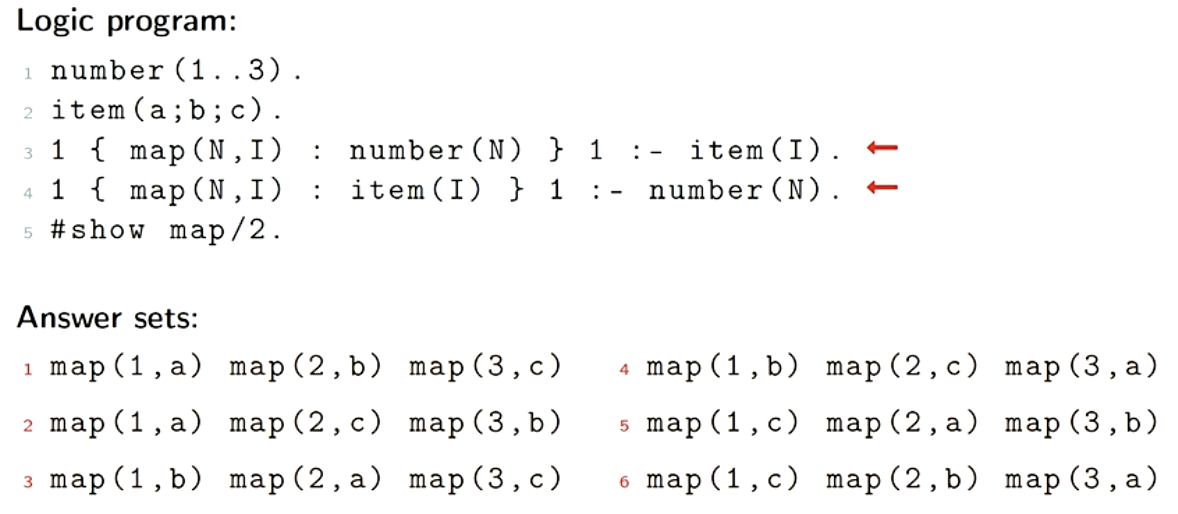
\includegraphics[scale=0.6]{figures/one-to-one.png}
\end{figure}

\newpage
\subsection{Generate and test}
Some useful \textcolor{Maroon}{general guidelines} for modelling a problem in ASP:
\begin{itemize}
    \item Seperate the \textcolor{MidnightBlue}{input} (the encoding of the problem input) from the \textcolor{MidnightBlue}{problem} (the encoding of the solution requirements).
    \item The \textcolor{MidnightBlue}{generate and test} approach.
\end{itemize}

\vspace{0.5cm}

Both have 4 steps:
\begin{enumerate}
    \setlength\itemsep{-0.25em}
    \item \textbf{Formalize the problem}
    \begin{itemize}
        \setlength\itemsep{-0.25em}
        \item What is the \textcolor{Maroon}{problem input}?
        \item What kind of objects are (candidate) solutions?
        \item What properties do solutions need to have?
    \end{itemize}
    \item \textbf{Establish encoding of problem instances}
    \begin{itemize}
        \setlength\itemsep{-0.25em}
        \item What predicates to use to represent the \textcolor{Maroon}{problem input}? What is their arity?
        \item What constants to use to represent the \textcolor{Maroon}{problem input}?
        \item How to translate the \textcolor{Maroon}{problem input} to facts that use these predicates and constants.
    \end{itemize}
    \item \textbf{Establish encoding of candidate solutions (\textcolor{MidnightBlue}{generate})}
    \begin{itemize}
        \setlength\itemsep{-0.25em}
        \item What predicates to use to represent \textcolor{Maroon}{candidate solutions}? What is their arity?
        \item What rules/constraints to add so that the answer sets of the program correspond to all \textcolor{Maroon}{candidate solutions}?
        \item Do you need any auxiliary predicates/rules to express some properties that \textcolor{Maroon}{candidate solutions} should have?
        \item How to obtain from any answer set the corresponding \textcolor{Maroon}{candidate solution}?
    \end{itemize}
    \item \textbf{Establish encoding of solution properties (\textcolor{MidnightBlue}{test})}
    \begin{itemize}
        \setlength\itemsep{-0.25em}
        \item What rules/constraints to add so that only the answer sets remain that correspond to \textcolor{Maroon}{actual solution}?
        \item Do you need any auxiliary predicates/rules to express some properties that \textcolor{Maroon}{actual solutions} should have?
    \end{itemize}
\end{enumerate}

\newpage
\textbf{Example:} 
\begin{figure}[ht!]
    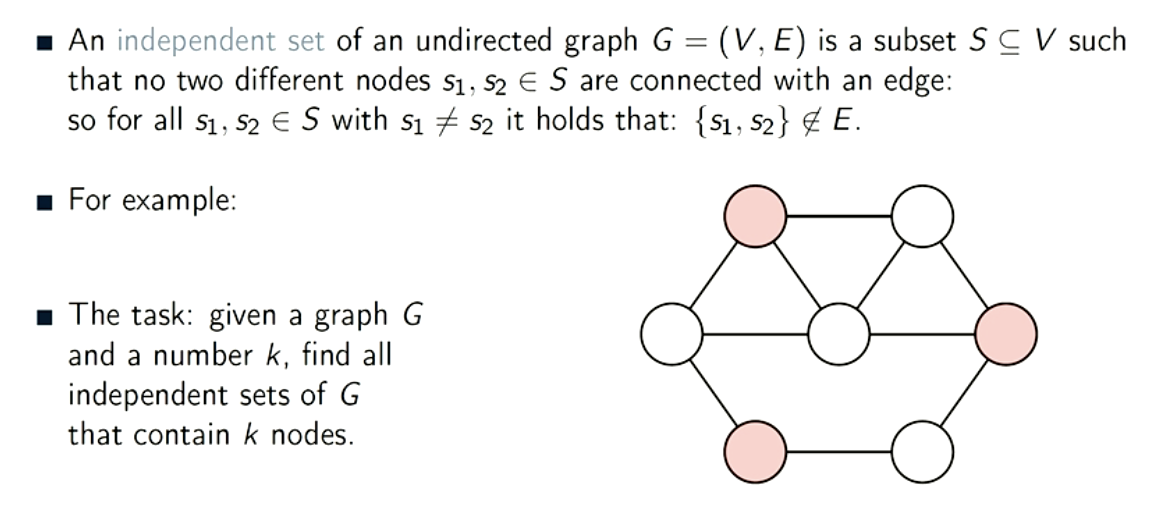
\includegraphics[scale=0.6]{figures/example 1.png}
\end{figure}


\begin{minipage}{0.5\textwidth}
    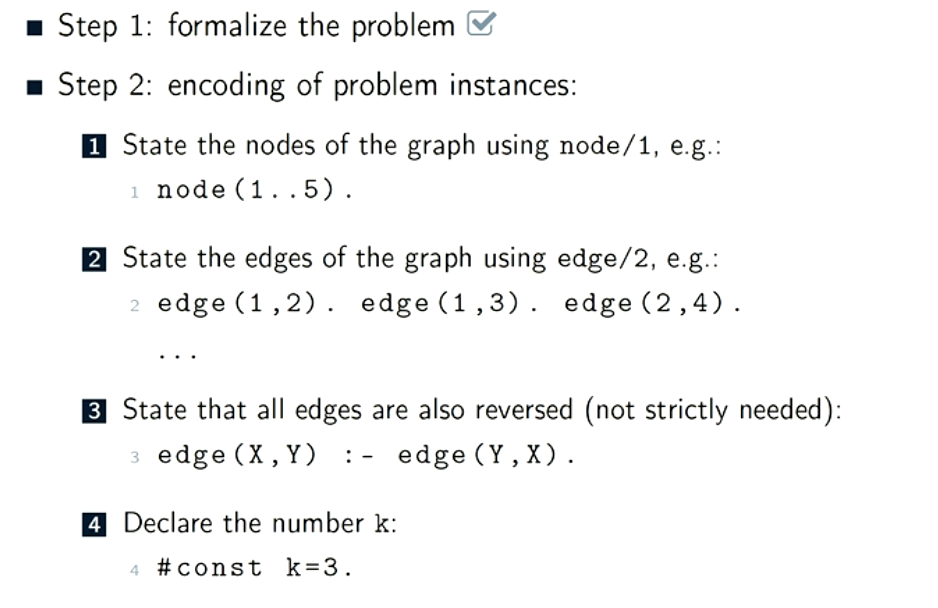
\includegraphics[scale=0.5]{figures/example 2.png}
\end{minipage}
\begin{minipage}{0.5\textwidth}
    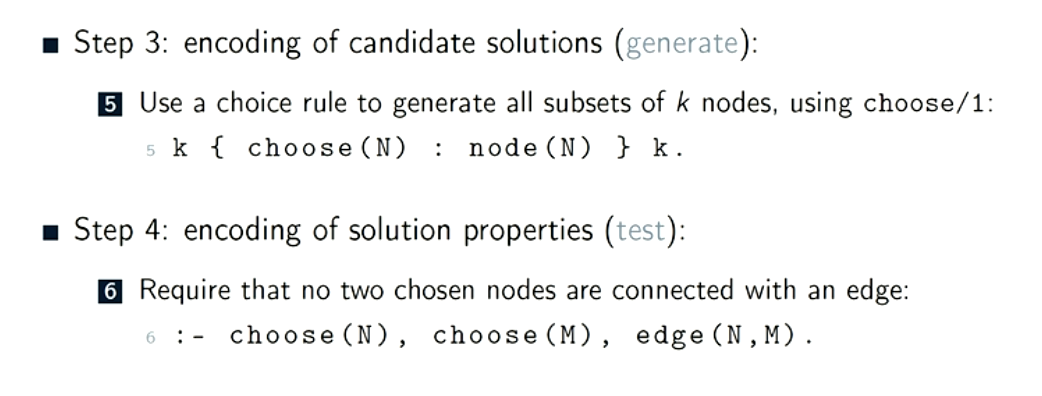
\includegraphics[scale=0.5]{figures/example 3.png}
\end{minipage}

\subsection{Grounding}
{\Large \textbf{\textcolor{Maroon}{Grounding algorithm}}}:
\begin{itemize}
    \setlength\itemsep{-0.25em}
    \item Keep track of a set $D$ of atoms that appear in the head of some ground rule. Initially, $D$ contains the facts of the program $P$.
    \item Apply the following procedure, until $D$ does not change anymore:
    \begin{itemize}
        \setlength\itemsep{-0.25em}
        \item If there is a ground version of some rule in $P$ where all non-negated atoms in the body appear in $D$, add the head of the rule to $D$.
    \end{itemize}
    \item For example:
    \begin{lstlisting}
    path(a,b).
    path(b,c).
    path(X,Z) :- path(X, Y), path(Y,Z).
    \end{lstlisting}
    \begin{itemize}
        \setlength\itemsep{-0.25em}
        \item initially, \textcolor{MidnightBlue}{$D = \{\text{ path}(a,b). \text{ path}(b,c) \; \}$}
        \item One instantiation with atoms in $D$: \textcolor{MidnightBlue}{$\text{path}(a,c) \text{ :- } \text{path}(a,b), \text{ path}(b,c).$}
        \item Then, \textcolor{MidnightBlue}{$D = \{ \text{ path}(a,b). \text{ path}(b,c). \text{ path}(a,c) \;  \}$}, and the algorithm stops.
    \end{itemize}
\end{itemize}

\newpage
{\Large \textbf{\textcolor{Maroon}{Safety}}}: \\
To carry out this 'on demand' grounding, all rules and constraints need to have a property of \textcolor{Maroon}{safety}:
\begin{itemize}
    \item A rule/constraint is called \textcolor{Maroon}{safe} if every variable appearing in it appears at least once in the body in an unnegated literal.
\end{itemize}

\textbf{Examples}:  \\
Safe:
\begin{lstlisting}
a(X,Y,Z) :- b(X,Y), c(X,Z), not d(X,Y,Z)
\end{lstlisting}

Not safe:
\begin{lstlisting}
a(X,Y,Z) :- b(X,Y) not d(X,Y,Z)
\end{lstlisting}

Not safe (be careful with negated statements):
\begin{lstlisting}
a(X,Y,Z) :- b(X,Y), X + Y != Z $\textcolor{PineGreen}{\text{\;\;\;\; \# Z is unsafe here}}$
\end{lstlisting}